%\documentclass{amsart}

% Packages

\usepackage{epstopdf}
\usepackage{amsmath, amssymb, amsthm}
%\usepackage[right=3cm,left=3cm,marginparwidth=2.5cm, marginparsep=0.5cm]{geometry}
\usepackage{enumitem}
\setlist[enumerate]{label=\text{\textnormal{(\alph*)}}}
\usepackage[toc,page]{appendix}
\usepackage{dsfont}
\usepackage{bbm}
\usepackage{url}
\usepackage{hyperref}
\usepackage[bottom]{footmisc}
\usepackage{footnote}
\usepackage{marginnote}
\usepackage{threeparttablex}
\usepackage{fmtcount}
\usepackage[usenames,dvipsnames,svgnames,table]{xcolor}
\usepackage[all,cmtip]{xy}
\let\objectstyle=\displaystyle
\usepackage[noabbrev,nameinlink]{cleveref}
\usepackage{tikz}
\usepackage{tkz-fct}
\usepackage{pgfplots}
\usepackage{graphicx}
\usepackage[lite]{amsrefs}

% Equation Options

\numberwithin{equation}{section}

% Libraries

\usetikzlibrary{matrix}
\usetikzlibrary{arrows}
\usetikzlibrary{decorations.pathmorphing}
\usetikzlibrary{trees}

% Theorem Environments

\newtheorem*{wrn}{Warning}
\newtheorem{thm}{Theorem}
\numberwithin{thm}{section}
\newtheorem{lem}[thm]{Lemma}
\newtheorem{prop}[thm]{Proposition}
\newtheorem{cor}[thm]{Corollary}
\newtheorem{claim}{Claim}
\theoremstyle{definition}
\newtheorem{problem}{Problem}
\newtheorem{case}{Case}
\newtheorem{defn}{Definition}
\numberwithin{defn}{section}
\newtheorem{ntn}{Notation}
\numberwithin{ntn}{section}
\newtheorem{conj}{Conjecture}
\numberwithin{conj}{section}
\newtheorem{exmp}{Example}
\numberwithin{exmp}{section}
\newtheorem{exmps}[exmp]{Examples}
\newtheorem{counter}[exmp]{Counterexample}
\newtheorem{rem}{Remark}
\numberwithin{rem}{section}
\theoremstyle{remark}



\begin{document}

\begin{figure}
\centering
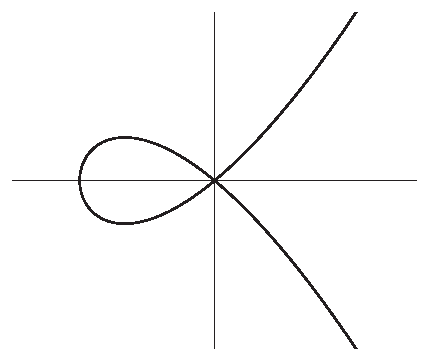
\includegraphics[width=0.4\linewidth]{Node/Node}
\caption{A node with equation $ y^{2} = x^{3} + x $. The file for this image is \texttt{Node.pdf}.}
\label{fig:Node}
\end{figure}

\begin{figure}
\centering
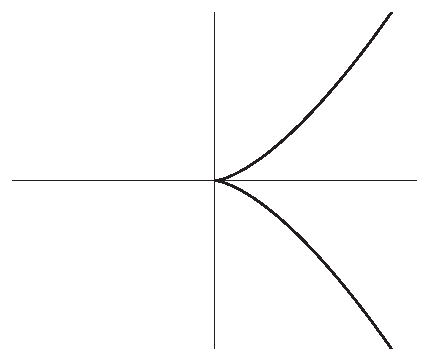
\includegraphics[width=0.4\linewidth]{Cusp/Cusp}
\caption{A cusp with equation $ y^{2} = x^{3} $. The file for this image is \texttt{Cusp.pdf}.}
\label{fig:Cusp}
\end{figure}


\begin{figure}
\centering
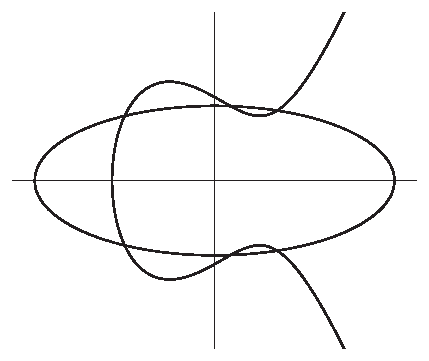
\includegraphics[width=0.4\linewidth]{Intersecting/Intersecting}
\caption{An ellipse intersecting a curve in 6 points. The ellipse has equation $ x^{2} + 4 y^{2} = 16 $ and the curve has equation $ y^{2} = x^{3} - 3 x + 5 $. The file for this image is \texttt{Intersecting.pdf}.}
\label{fig:Intersecting}
\end{figure}


\begin{figure}
\centering
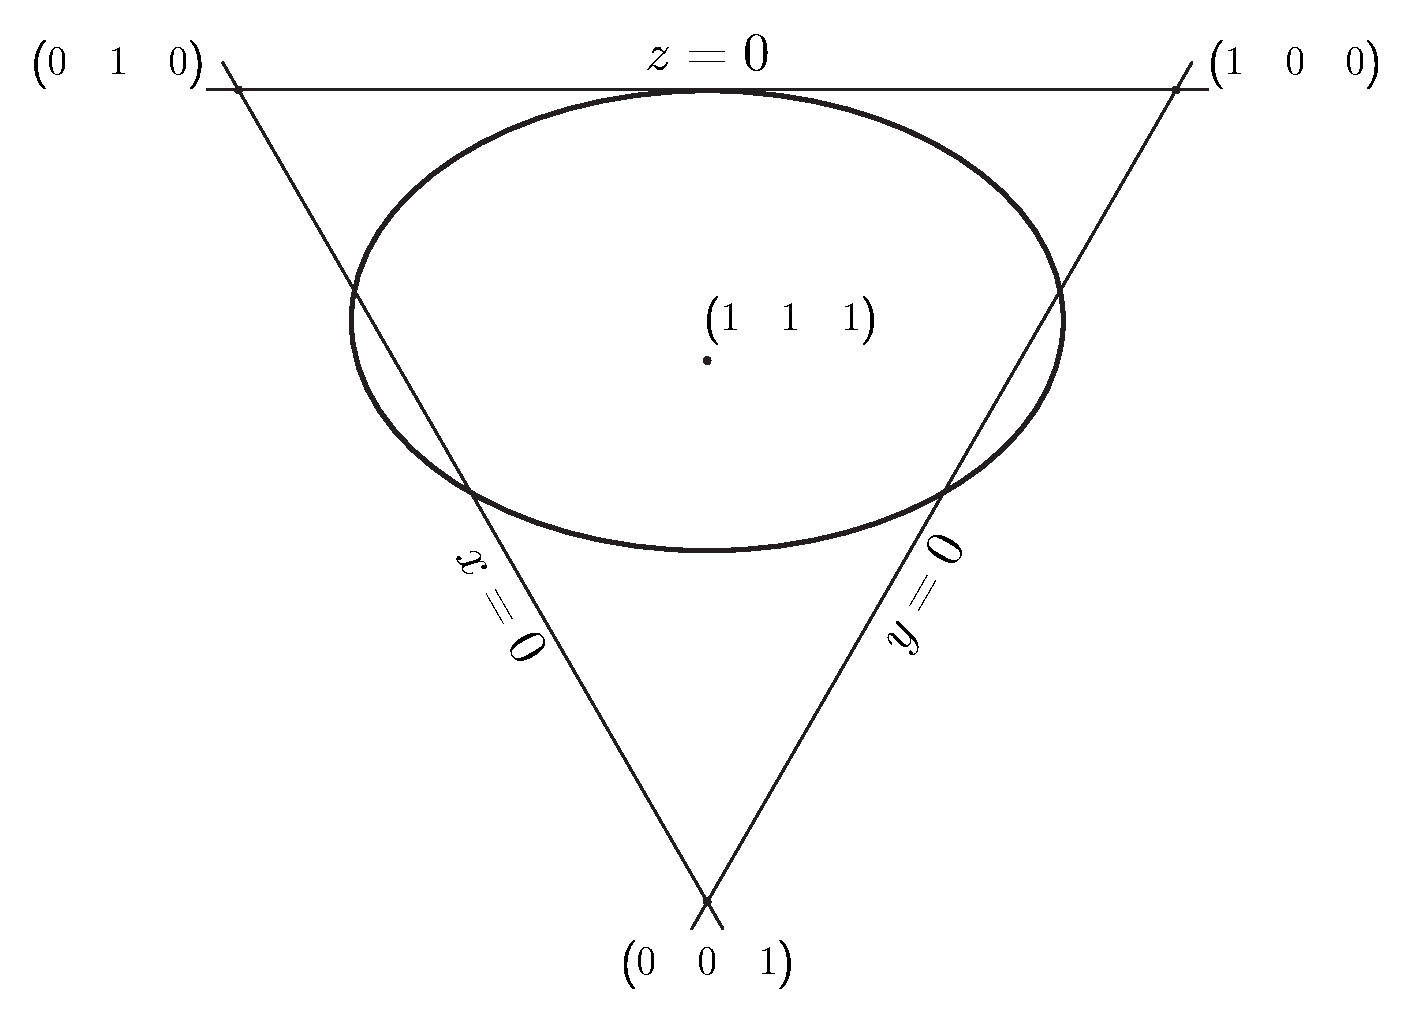
\includegraphics[width=0.7\linewidth]{Plane/Plane}
\caption{An ellipse with projective coordinate equation $ (x - y)^{2} + z(3z - 4x - 4y) = 0 $. The file for this image is \texttt{Plane.pdf}.}
\label{fig:Plane}
\end{figure}

\begin{figure}
\centering
\includegraphics[width=0.6\linewidth]{Projecting/Projecting}
\caption{Projecting from $ \mathbb{P}^{2} $ to $ \mathbb{P}^{1} $. The ellipse in is picture is the same as the one in the previous picture. The file for this image is \texttt{Projecting.pdf}.}
\label{fig:Projecting}
\end{figure}


 
\end{document}